\section{Overview}

\subsection{A Story in Pictures}
\begin{frame}
  \centering
  
\includegraphics[height=0.95\textheight]{phd1531}
  \footnote{http://phdcomics.com/comics/archive.php?comicid=1531}
\end{frame}

\begin{frame}
  \centering
  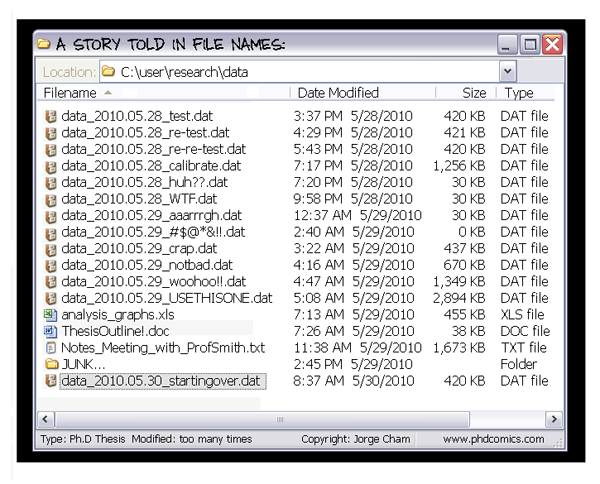
\includegraphics[height=0.95\textheight]{phd1323}
  \footnote{http://phdcomics.com/comics/archive.php?comicid=1323}
\end{frame}

\subsection{Tracking History}

\begin{frame}
  \frametitle{Tracking Changes}
  \begin{itemize}
    \item The history of a project can be viewed as a series of changes:
      \begin{itemize}
        \item A unique identifier
        \item What changed?
        \item When did it change?
        \item Who changed it?
        \item Why did it change?
      \end{itemize}
    \item[]
    \item Difficult to manually track multiple files
  \end{itemize}
\end{frame}

\begin{frame}
  \frametitle{Git: A Version Control System}
  A snapshot of the working directory is taken and \emph{commit}ted to the git data base.
  \begin{itemize}
    \item Unique identifier
      \begin{itemize}
        \item SHA-1 (determined by the files, the author, date, description of change, and the prior history)
      \end{itemize}
    \item What changed \begin{itemize} \item  git diff \end{itemize}
    \item Who changed it \begin{itemize} \item git blame \end{itemize}
    \item Why did it change \begin{itemize} \item git log \end{itemize}
    \item[]
    \item for example:
  \end{itemize}
\end{frame}

\begin{frame}[t,fragile]
  \tiny
  \inputminted{text}{eglog.log}
\end{frame}

\begin{frame}[t,fragile]
  \frametitle{What changed?}
  \small
  \inputminted{text}{egdiff}

  \normalsize
  \begin{itemize}
    \item Diffs are easier to see in several GUI thanks to color coding. More on
      this later.
  \end{itemize}
\end{frame}

\begin{frame}[t,fragile]
  \frametitle{Skipping over errors}
  \small
  \inputminted[firstline=1,lastline=10]{text}{eglog.log}
\end{frame}

\subsection{Overview of Git}

\begin{frame}
  \frametitle{Conceptual Git and Version Control}
  \begin{itemize}
    \item Local Version Control
    \item Centralized Version Control System
    \item Distributed Version Control System
    \item Short History and Design of Git
  \end{itemize}
\end{frame}

\begin{frame}
  \frametitle{Local Version Control System}
  \centering
  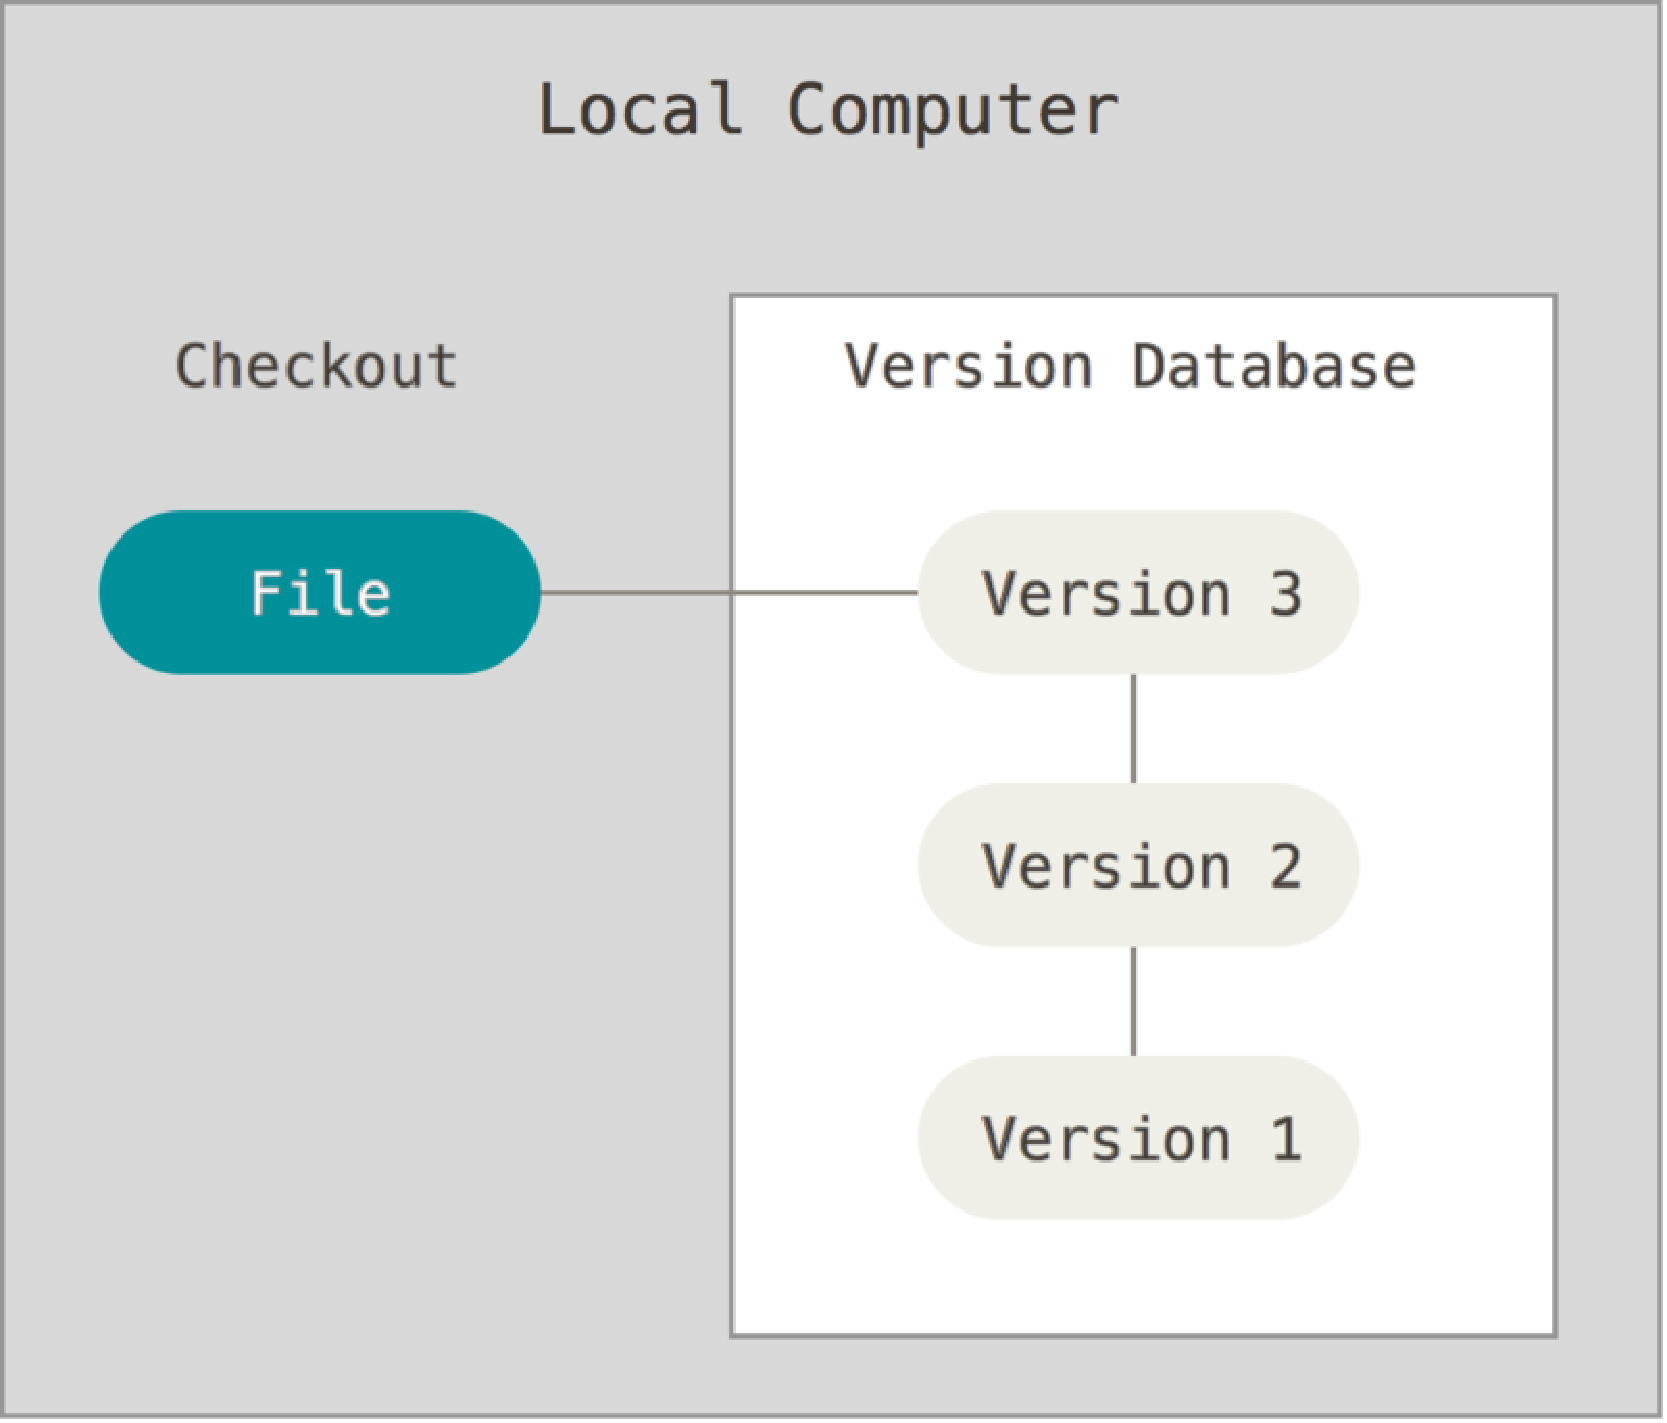
\includegraphics[height=0.80\textheight]{local-vcs}
  \footnote{https://git-scm.com/book/en/v2/Getting-Started-About-Version-Control}
\end{frame}

\begin{frame}
  \frametitle{Centralized Version Control System}
  \centering
  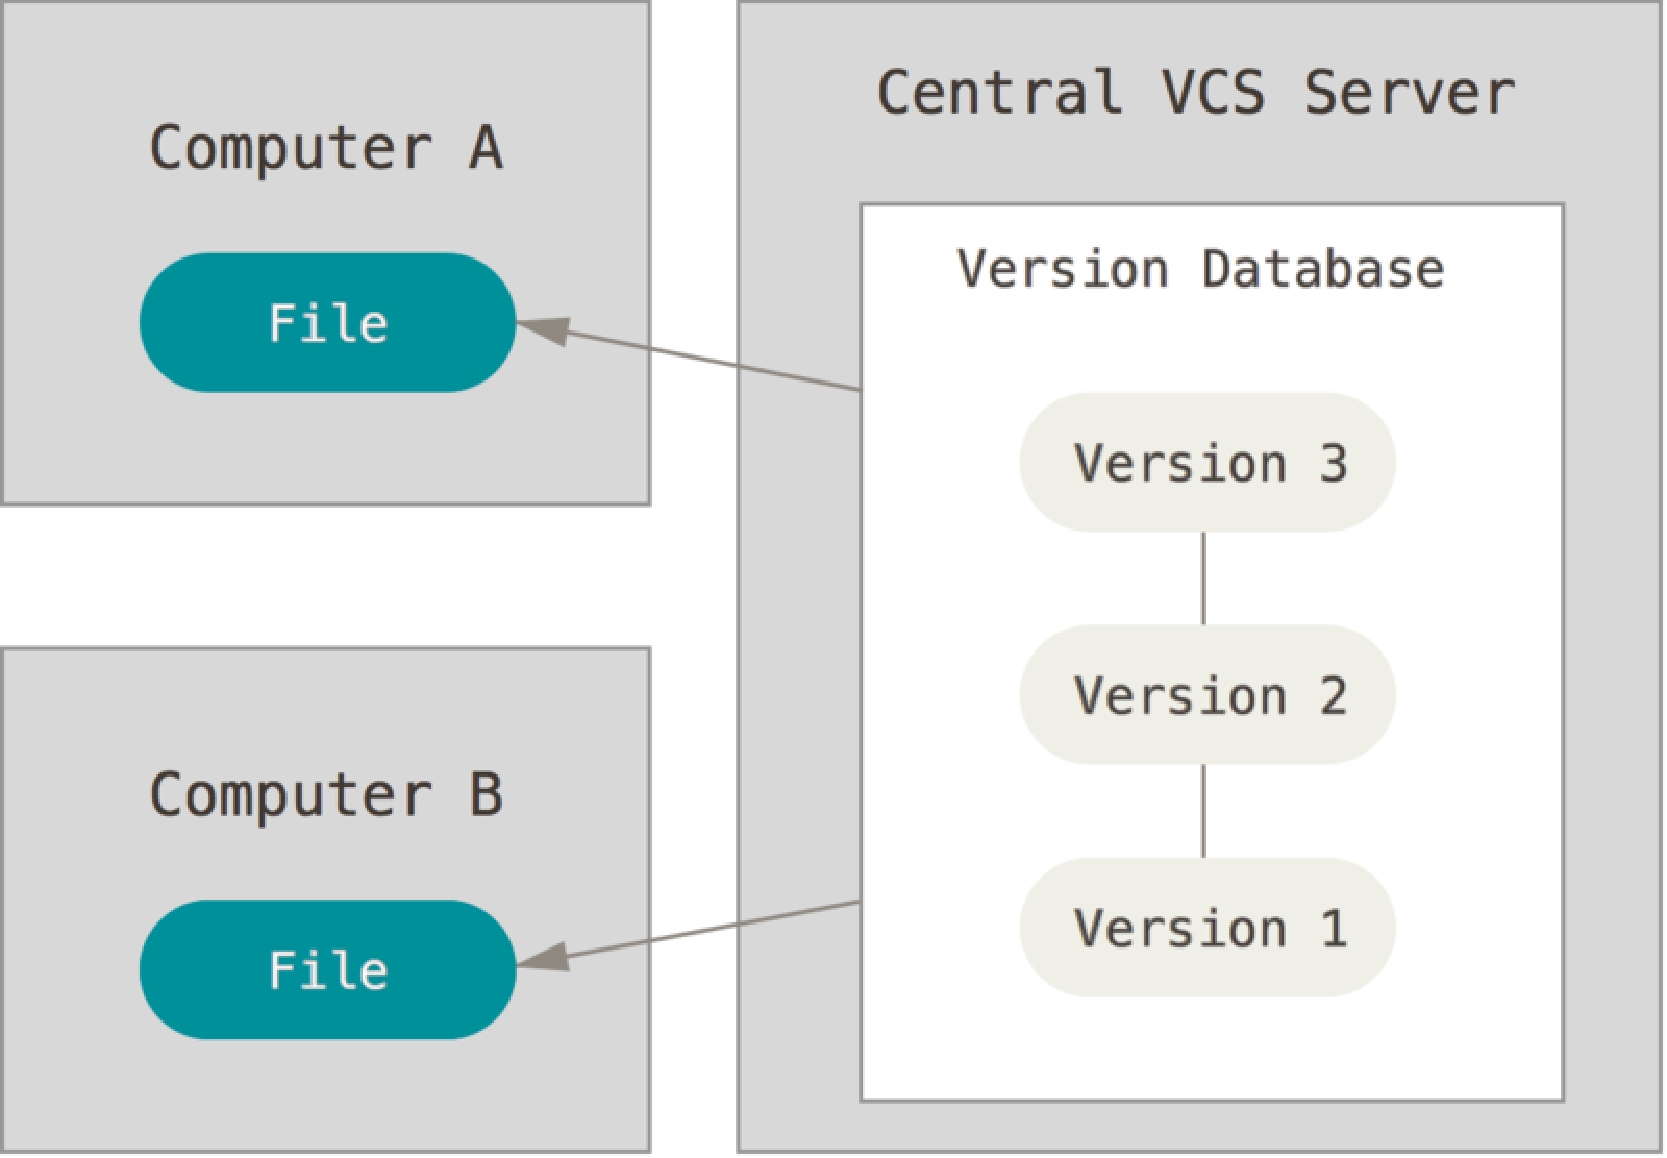
\includegraphics[height=0.80\textheight]{centralized-vcs}
  \footnote{https://git-scm.com/book/en/v2/Getting-Started-About-Version-Control}
\end{frame}

\begin{frame}
  \frametitle{Distributed Version Control System}
  \centering
  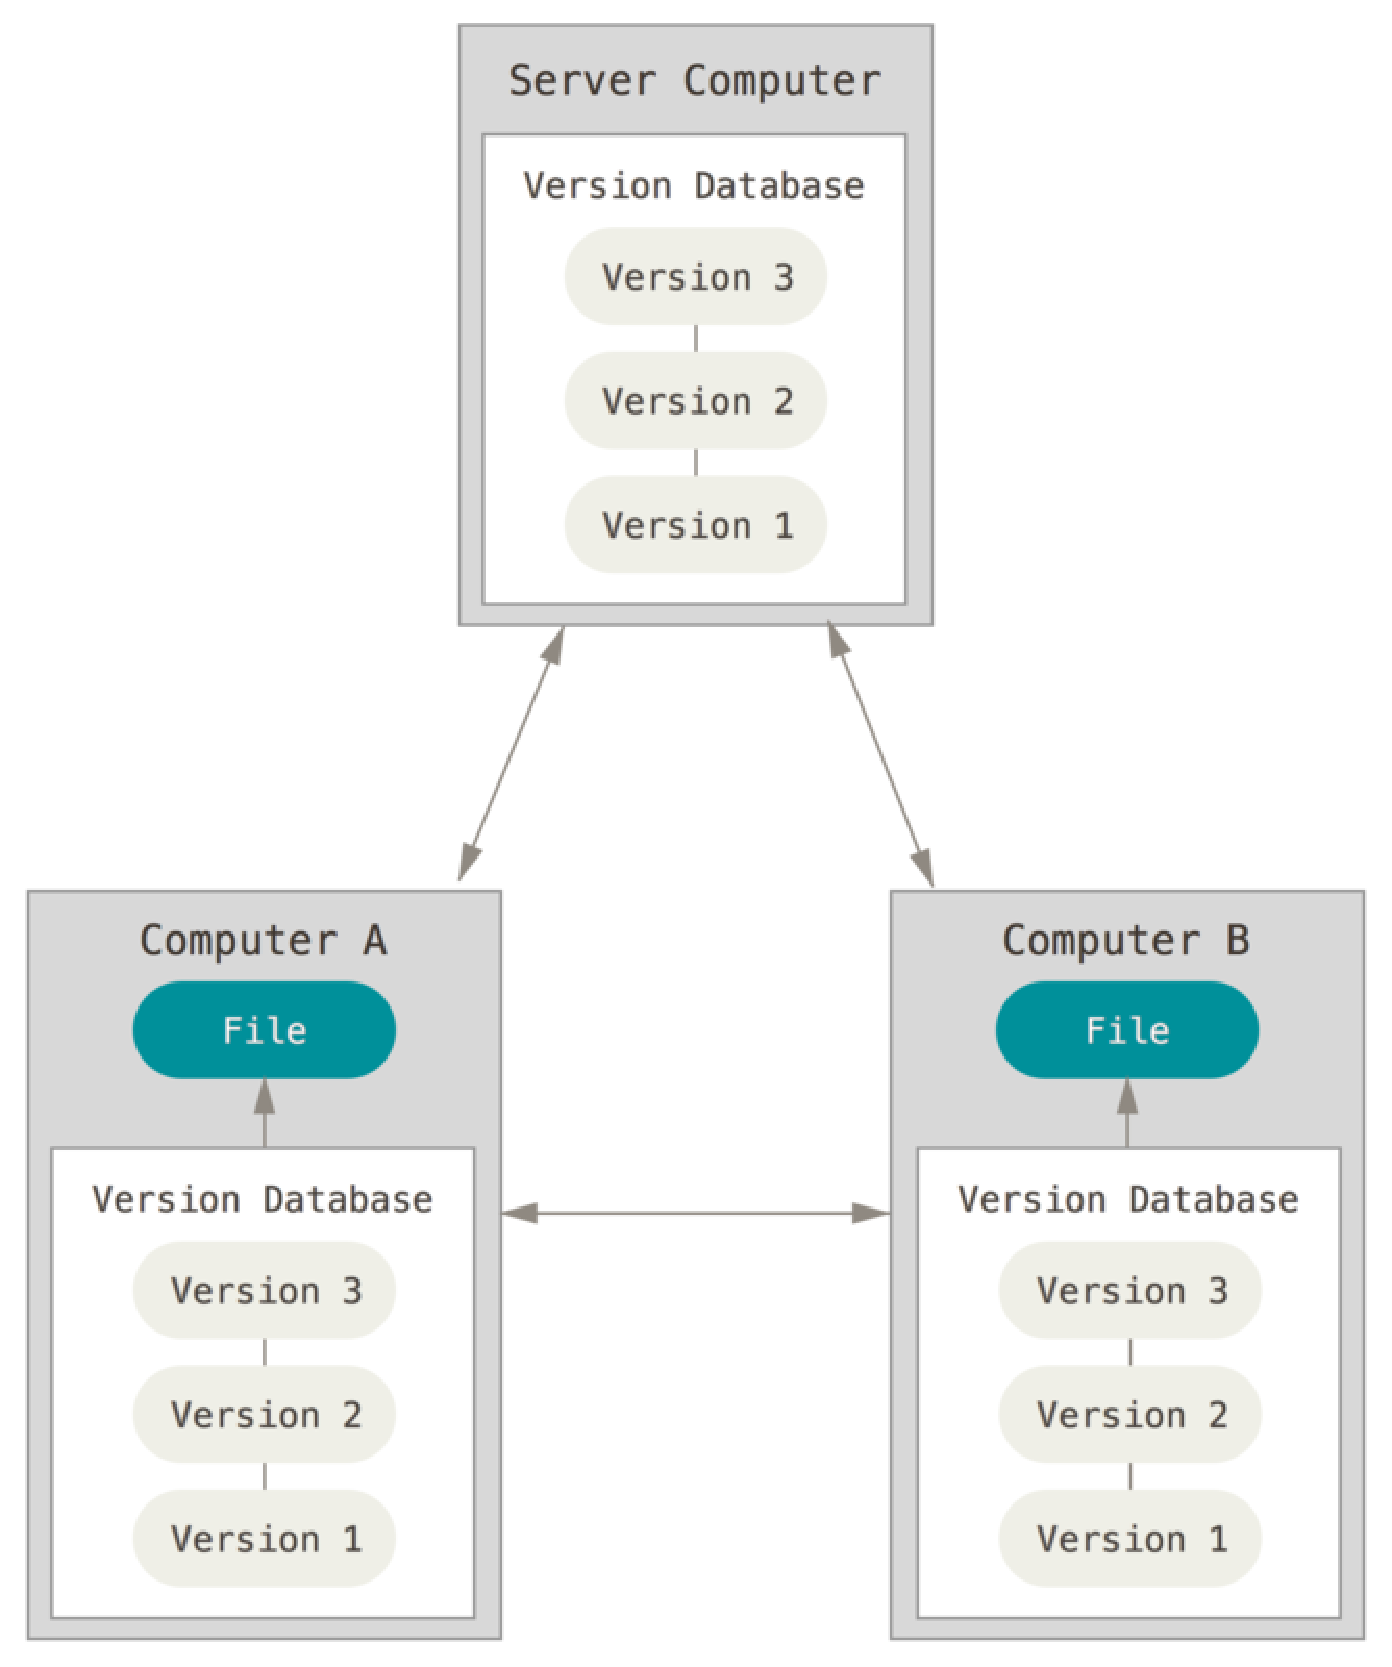
\includegraphics[height=0.80\textheight]{distributed-vcs}
  \footnote{https://git-scm.com/book/en/v2/Getting-Started-About-Version-Control}
\end{frame}

\begin{frame}
  \frametitle{Short History of Git}
  \begin{itemize}
    \item Original Author: Linus Torvalds
    \item Version 0.99 released July 2005
    \item Current version 2.24
    \item Linux vs BitKeeper
    \item Linux dev community sets out to develop their own DVCS with the
      goals of:
      \begin{itemize}
        \item speed
        \item simple design
        \item strong support for non-linear development (thousands of parallel
          branches)
        \item fully distributed
        \item able to handle large projects, line the Linux kernel, efficiently
      \end{itemize}
  \end{itemize}
\end{frame}

\begin{frame}
  \frametitle{Snapshots; Not Differences}
  \centering
  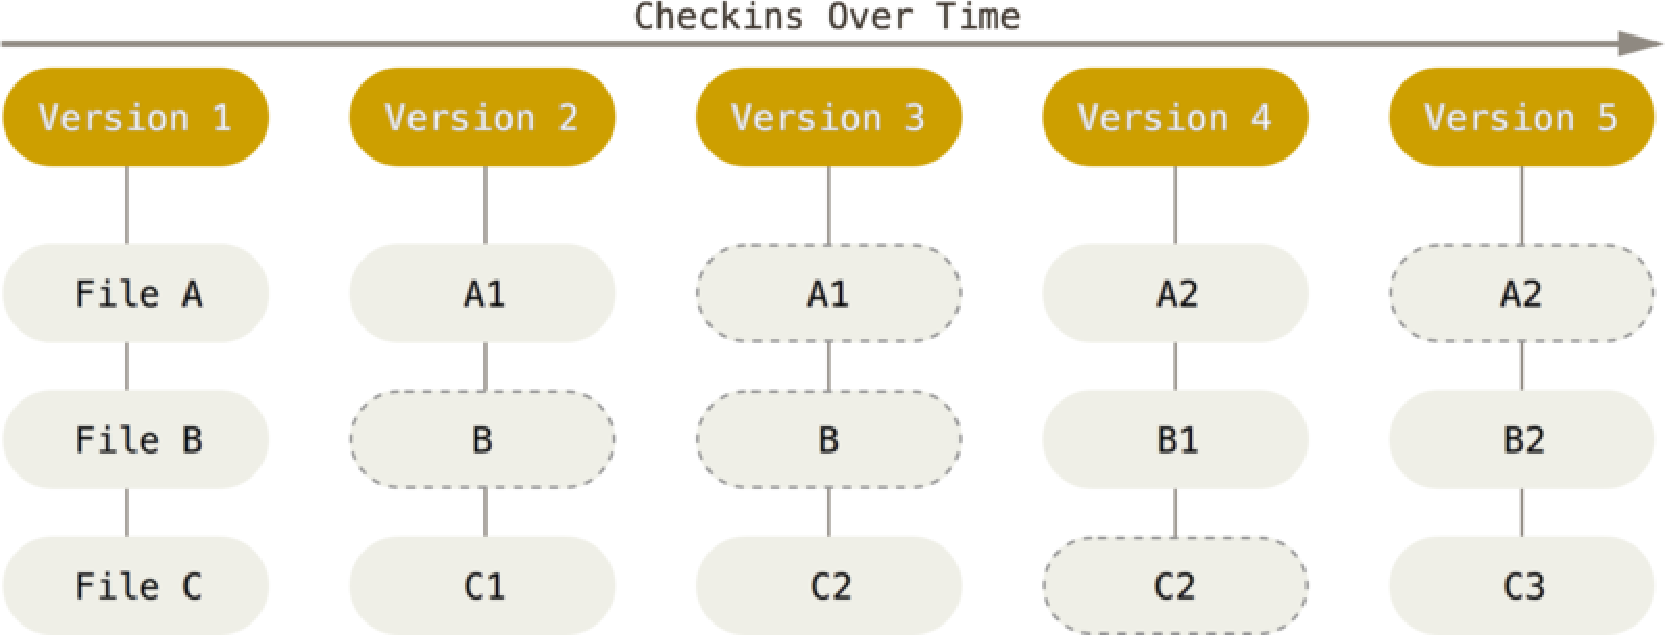
\includegraphics[width=0.90\textwidth]{snapshots}
  \footnote{https://git-scm.com/book/en/v2/Getting-Started-What-is-Git\%3F}
\end{frame}

\begin{frame}
  \frametitle{Nearly Every Operation is Local}
  \begin{itemize}
    \item Most operations are local
      \begin{itemize}
        \item No need to talk to other computers on a network
        \item The entire project history is on your local machine
      \end{itemize}
    \item You can work off vpn
    \item You can work offline
  \end{itemize}
\end{frame}

\begin{frame}
  \frametitle{Git Has Integrity}
  \begin{itemize}
    \item Everything is check-summed (remember the sha?)
    \item You cannot lose information in transit nor get a file corruption
      without git being able to detect it
    \item git stores everything in its database not by file name but by the hash
      value of its contents
    \item git has been designed for multiple parallel development, i.e.,
      multiple programmers contributing to one project non-linearly in time
  \end{itemize}
\end{frame}

\begin{frame}
  \frametitle{Git Generally Only Adds Dat}
  \begin{itemize}
    \item Nearly all actions in git add data to the git database
    \item It is difficult to do anything that is not undoable
    \item You can lose/corrupt un-committed changes
    \item It is very difficult to lose anything after a commit, especially with
      frequent pushes to other repositories
  \end{itemize}
\end{frame}

\begin{frame}
  \frametitle{The Three Stages}
  \begin{itemize}
    \item Git has three main states that files reside in
      \begin{itemize}
        \item Committed: data is safely stored in the local database
        \item Modified: changed the file(s) but have not committed to the
          data base yet
        \item Staged: marked modified files(s) in current version to go into the
          next commit snapshot
      \end{itemize}
    \item This leads to three main sections of a git project
      \begin{itemize}
        \item the .git directory
        \item the working directory
        \item the staging area
      \end{itemize}
  \end{itemize}
\end{frame}

\begin{frame}
  \frametitle{The Three Stages}
  \begin{center}
  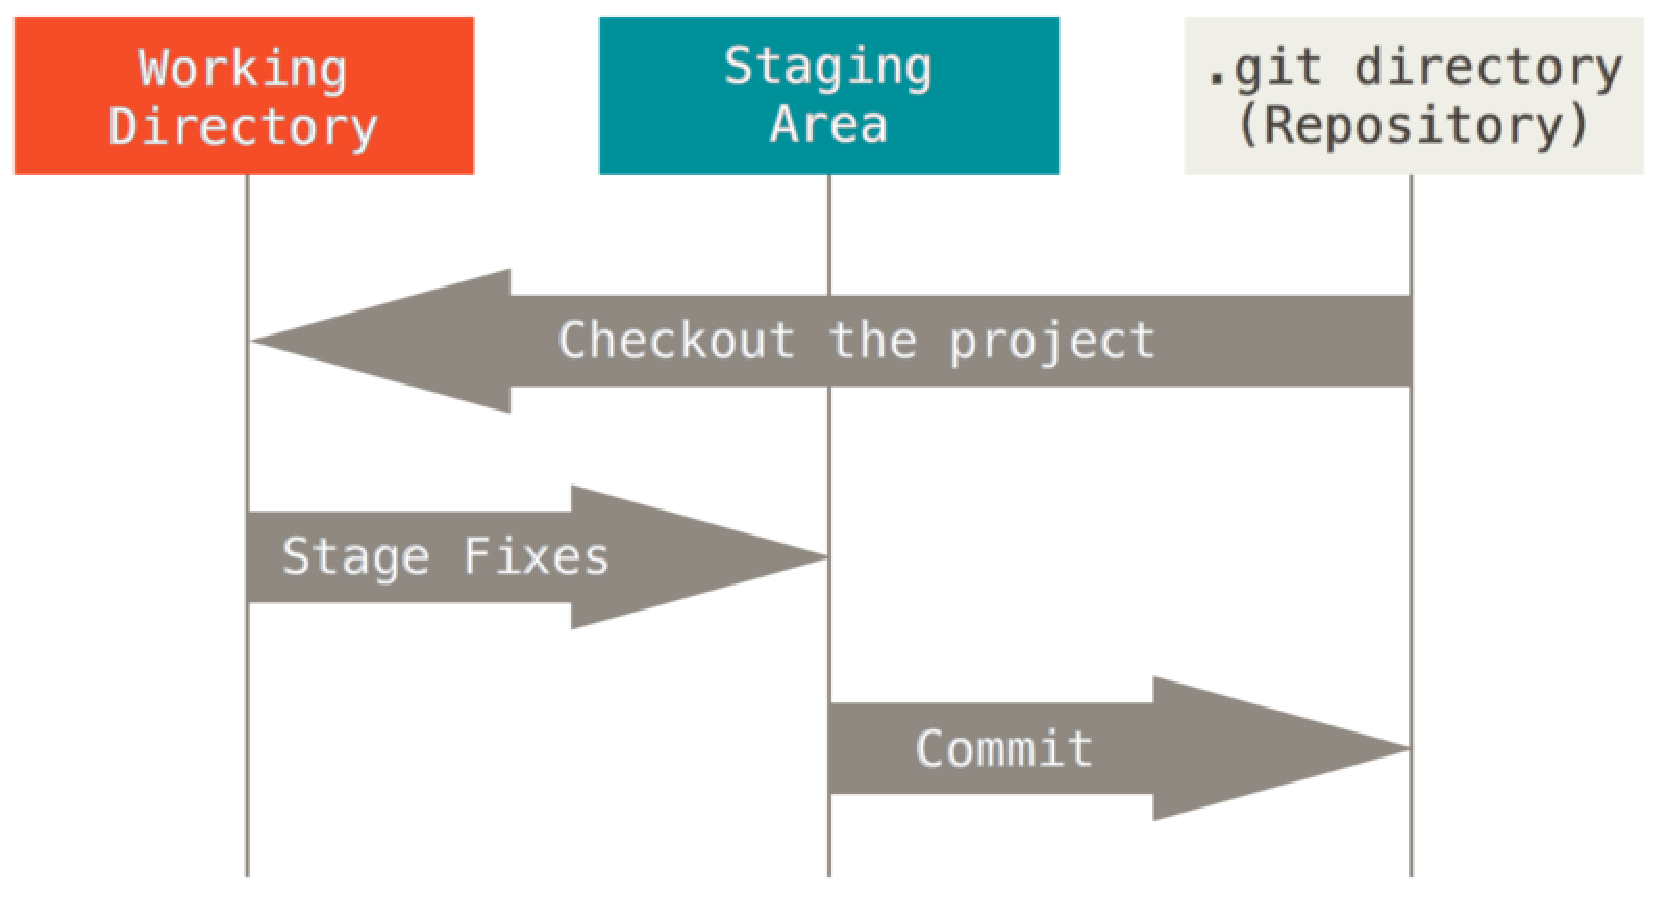
\includegraphics[width=0.5\textwidth]{areas}
  \end{center}

  Basic Git workflow
  \begin{itemize}
    \item Modify: make changes in the working directory
    \item Stage: adding snapshots to the staging area
    \item Commit: move the shapshot in the staging area to the .git database
  \end{itemize}
\end{frame}
